\item[(c)]
\section*{Task (c)}

\subsection*{Problem Statement}
After ideal reconstruction, you end up with the analog signals \( x_1(t) \) and \( x_2(t) \). Sketch the reconstructed analog spectra. Plot the reconstructed time-domain signal. Compare your results with Task (a).

\subsection*{Theoretical Background}
Ideal reconstruction involves passing the sampled signal through an ideal low-pass filter with a cutoff frequency equal to half the sampling frequency. This process removes any aliasing components and reconstructs the original analog signal.

For a signal sampled at frequency \( f_s \), the reconstructed signal will ideally contain frequency components up to \( f_s / 2 \). The original frequencies in \( x(t) \) must be within this range for perfect reconstruction.

\subsection*{Mathematical Derivation}
Given the sampling frequencies \( f_{s1} = 9 \, \text{kHz} \) and \( f_{s2} = 14 \, \text{kHz} \), the reconstructed signals \( x_1(t) \) and \( x_2(t) \) will contain frequency components up to 4.5 kHz and 7 kHz, respectively.

The ideal reconstructed spectra will be band-limited to the corresponding Nyquist frequencies:
- \( x_1(t) \): Frequencies up to 4.5 kHz
- \( x_2(t) \): Frequencies up to 7 kHz

\subsection*{Python Implementation and Plot}
The plot Figure~\ref{fig:ex1_c_reconstructed_x1} below illustrates the reconstructed time-domain signal \( x_1(t) \) sampled at 9 kHz, and Figure~\ref{fig:ex1_c_reconstructed_x2} shows the reconstructed time-domain signal \( x_2(t) \) sampled at 14 kHz:

\begin{figure}[h]
    \centering
    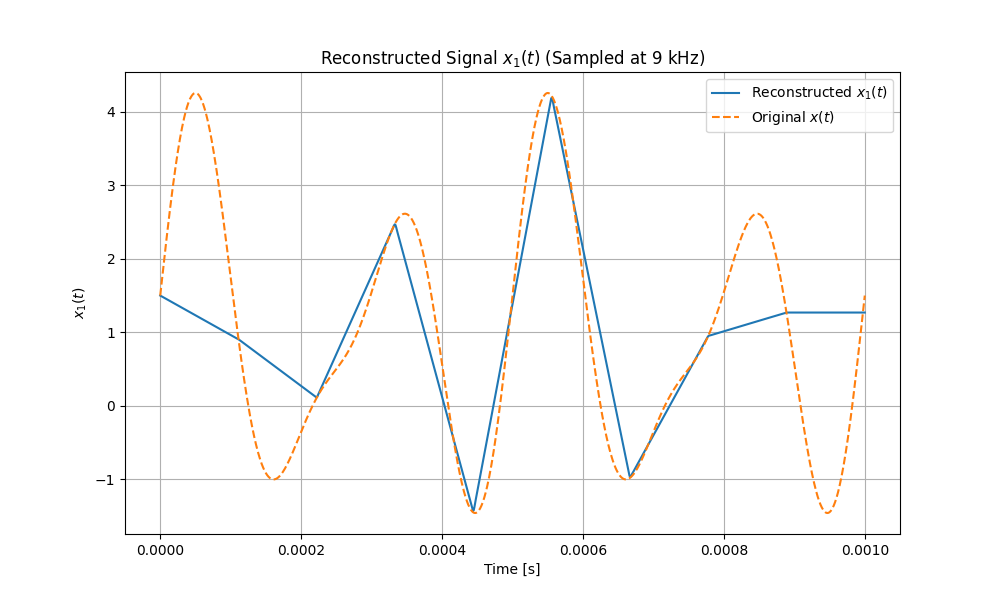
\includegraphics[width=0.8\textwidth]{fig/ex1_c_reconstructed_x1.png}
    \caption{Reconstructed Signal $x_1(t)$ (Sampled at 9 kHz)}
    \label{fig:ex1_c_reconstructed_x1}
\end{figure}

\begin{figure}[h]
    \centering
    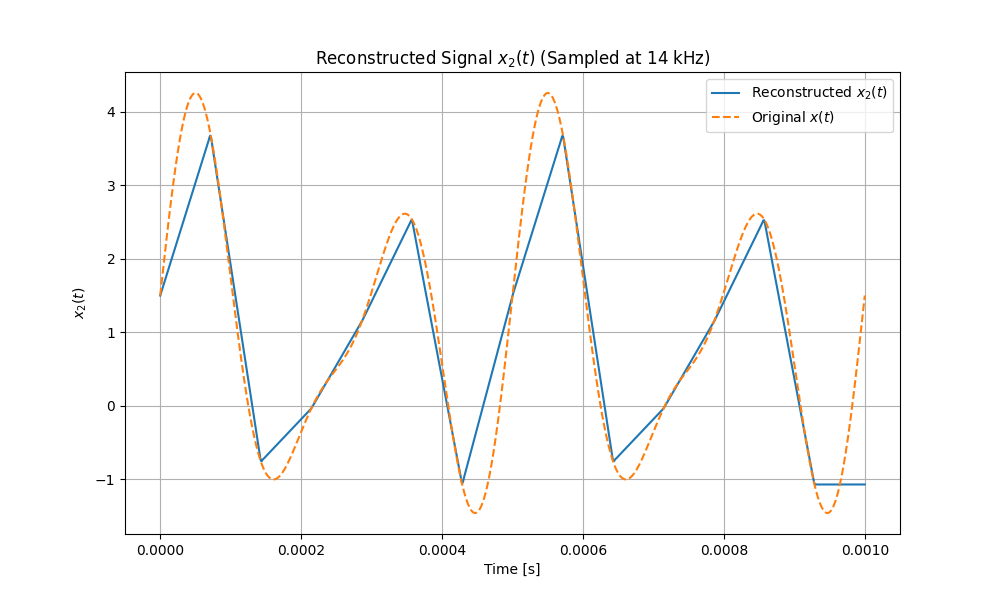
\includegraphics[width=0.8\textwidth]{fig/ex1_c_reconstructed_x2.png}
    \caption{Reconstructed Signal $x_2(t)$ (Sampled at 14 kHz)}
    \label{fig:ex1_c_reconstructed_x2}
\end{figure}

\subsection*{Conclusion}
The reconstructed signals \( x_1(t) \) and \( x_2(t) \) after ideal reconstruction show that the original signal can be accurately recovered when the sampling frequency is sufficiently high. The reconstructed time-domain signals closely match the original signal, demonstrating the effectiveness of ideal reconstruction.

Comparing the results with Task (a), we observe that the reconstructed signals \( x_1(t) \) and \( x_2(t) \) successfully capture the original signal's characteristics within the respective Nyquist limits of the sampling frequencies used.
